\usepackage{enumitem}

\iflatexml
\else
% reset fancyhr settings set by artisynthDoc
\fancyhead[L,C,R]{}
\fancyfoot[L,R]{}
\fancyfoot[C]{\thepage}
\renewcommand{\headrulewidth}{0pt}
\renewcommand{\footrulewidth}{0pt}
\fi

\def\ArtHome[#1]{{\tt <ARTISYNTH\_HOME>#1}}

\title{Installing ArtiSynth from GitHub into Eclipse (\SYSTEM{})}
\author{John Lloyd}
\setpubdate{Last updated: March, 2021}
\iflatexml
\date{}
\fi

\newif\ifNeedLibraryPath
\NeedLibraryPathfalse

\begin{document}

%\maketitle

\iflatexml{\large\pubdate}\fi

%\tableofcontents

% add title in PDF version
\iflatexml\else
\begin{center}
{\sffamily\Large\bfseries 
Installing ArtiSynth from GitHub into Eclipse (\SYSTEM{})}
\end{center}
\bigskip
\fi

\section{Overview}

This document describes how to install ArtiSynth directly from GitHub
and import it into the Eclipse IDE (Integrated Development
Environment), within a \SYSTEM{} environment. While for demonstration
purposes it is faster to install ArtiSynth using a precompiled
release, installing from GitHub provides access to the most recent
updates, and the Eclipse IDE is a convenient platform for developing
and modifying the Java code used to create ArtiSynth models.

There are three parts to the installation process:

\begin{enumerate}

\item Installing Java

\item Installing Eclipse

\item Installing ArtiSynth from GitHub

\end{enumerate}

Your host machine should be a 64 bit system that is based on the Intel
processor. ArtiSynth may also run on ARM-based systems that provide an
Intel compatibility layer.
%
\ifMacOS
\begin{sideblock}
The new Apple ARM-based systems provide an Intel compatibility layer,
named Rosetta, that appears to allow ArtiSynth to run as is.
\end{sideblock}
\fi
%
We recommend a minimum of 8 Gbytes of memory, and 16 Gbytes or more is
better if you are doing FEM work with larger numbers of elements.

%\ifMacOS 
%\begin{sideblock}
%{\bf Possible issues regarding ArtiSynth on MacOS:} First, Apple has
%deprecated OpenGL (which ArtiSynth uses for 3D graphics), and so it is
%not clear how long OpenGL will continue to be available.  While it is
%possible to retarget ArtiSynth onto a different graphics engine, this
%will require a fair amount of work.  Second, Apple is retiring the use
%of Intel-based processors, which ArtiSynth relies on for its sparse
%matrix solver. Fortunately, Apple ARM machines do currently implement
%an Intel compatibility layer (called Rosetta) that does appear to
%allow ArtiSynth to run as is.
%\end{sideblock}
%\fi

This document is intentionally brief and describes only installation
from Git into an Eclipse IDE. More complete instructions,
including how to create and add models, integrate external
models, and update ArtiSynth, are given in the
\ifLinux
\artisynthManual[installation/linuxInstallation]{linuxInstallation}%
{General Installation Guide}.
\fi
\ifWindows
\artisynthManual[installation/windowsInstallation]{windowsInstallation}%
{General Installation Guide}.
\fi
\ifMacOS
\artisynthManual[installation/macosInstallation]{macosInstallation}%
{General Installation Guide}.
\fi
Instructions for visualizing, navigating, editing
and simulating models are given in the 
\artisynthManual{uiguide}{ArtiSynth User Interface Guide}.
Instructions on how to {\it build} a model using Java are given in
the \artisynthManual{modelguide}{ArtiSynth Modeling Guide}.

\section{Installing Java}
\label{InstallingJava:sec}

ArtiSynth requires that you have a full Java development kit (JDK)
installed, which comes with a Java compiler; a simple run time
environment (JRE) will not be sufficient. 
By default, ArtiSynth is compiled to be compliant with Java 8. While
ArtiSynth will generally work under later Java versions, use
of both the MATLAB and Jython interfaces generally requires Java 8.
Therefore we currently recommend using Java
8; this also provides maximum compatibility with MATLAB.
We specifically recommend the Java SE Development Kit 8u{\it
XXX} (where {\it XXX} is the latest revision number), which can be
obtained from Oracle (registration required).  At the time of this
writing, the download page is located at

\href{https://www.oracle.com/java/technologies/javase/javase-jdk8-downloads.html}%
{www.oracle.com/java/technologies/javase/javase-jdk8-downloads.html}

and the latest release is {\tt 8u281}. This page provides downloads
for all systems; be sure to choose the download link appropriate to
yours.
\ifWindows
For \SYSTEM{}, this will be {\tt jdk-8u281-windows-x64.exe}.  After
the file downloads, open it, and follow the installation wizard, using
the default values provided. The installer will probably install {\it
both} a JRE and a JDK, and place them in the \directories{}
\begin{verbatim}
C:\Program Files\Java\jre1.8.0_281
C:\Program Files\Java\jdk1.8.0_281
\end{verbatim}
The second contains the JDK, and is your {\it JDK installation} \directory{}.
\fi
\ifMacOS
For \SYSTEM{}, this will be {\tt jdk-8u281-macosx-x64.dmg}
After the file downloads, open it, and follow the installation instructions.
\fi

The {\tt java} and {\tt javac} commands associated with your Java 8
JDK must be visible from a terminal window. To verify this, open a
terminal window, run the command {\tt javac
-version}, and check that the command is found and that the version
matches the JDK.  If it does not, follow the instructions in Section
\ref{MakingJDKVisible:sec}.

\section{Installing Eclipse}

Eclipse is an integrated development environment (IDE) that is
commonly used for writing and maintaining Java programs. While other
IDEs exist for Java, such as NetBeans and IntelliJ, Eclipse is
currently the most commonly used amongst ArtiSynth users. It should be
noted, however, that an IDE is not {\it required} for Java
programming; simpler programs, in particular, can often be created by
editing the {\tt .java} source files using a text editor and then
compiling them with command line tools, including the {\tt compile}
utility supplied by ArtiSynth.

This document describes specifically the installation of Eclipse
2020-12; other versions should be similar.

Eclipse can be downloaded from
\href{https://www.eclipse.org/downloads/packages}%
{www.eclipse.org/downloads/packages}. From this page, choose ``{\sf
Eclipse IDE for Java Developers}'',
\ifWindows
{\sf Windows x86\_64}, which will download the file
\begin{verbatim}
  eclipse-java-2020-12-R-win32-x86_64.zip
\end{verbatim}
Unzip this into a convenient \directory{}, such as for example:
\begin{verbatim}
  C:\eclipse\eclipse-2020-12
\end{verbatim}
Open this \directory{}with a file explorer, and you will see the eclipse
application:

\begin{center}
   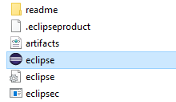
\includegraphics[width=0.25\textwidth]{images/EclipseApp}
\end{center}

Click on this to open it. 
\fi
\ifMacOS
{\sf macOS x86\_64}, which will download the file
\begin{verbatim}
  eclipse-java-2020-12-R-macosx-cocoa-x86_64.dmg
\end{verbatim}
Open this file, click on the ``Eclipse Installer'',
select ``Eclipse IDE for Java Developers'', and follow
the install instructions. When the install is complete,
click the {\sf Launch} button.
\fi
\ifLinux
{\sf Linux x86\_64}, which will download the file
\begin{verbatim}
  eclipse-java-2020-12-R-linux-gtk-x86_64.tar.gz
\end{verbatim}
Untar this file into any desired install location,
and then run the {\tt eclipse} executable in the
top-level directory.
\fi
The following dialog will appear,
asking you to select a workspace \directory:

\begin{center}
\iflatexml
  \ifWindows
     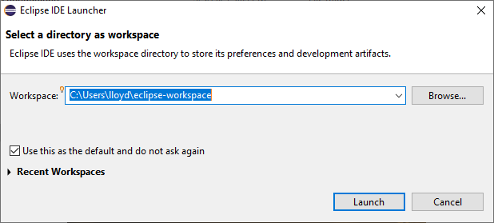
\includegraphics[]{images/EclipseWorkspaceDialog}
  \else
    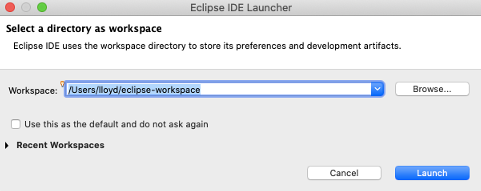
\includegraphics[]{images/EclipseWorkspaceDialogMacOS}
  \fi
\else
  \ifWindows
     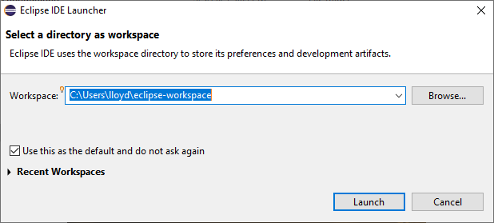
\includegraphics[width=0.7\textwidth]{images/EclipseWorkspaceDialog}
  \else
    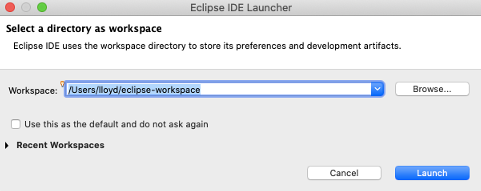
\includegraphics[width=0.7\textwidth]{images/EclipseWorkspaceDialogMacOS}
  \fi
\fi
\end{center}
This is where Eclipse settings and project information will be
stored. Unless you have a another Eclipse already installed, the
default location should be fine. (Remember also to check the ``{\sf
Use this as the default ...}''  box so that this query won't appear
every time you open Eclipse.) 
Next, click {\sf Launch}.  A welcome
page will appear; close this. A ``donate'' panel may also appear;
close this too.  You should then see an empty Eclipse display, similar
to this:

\begin{center}
\iflatexml
   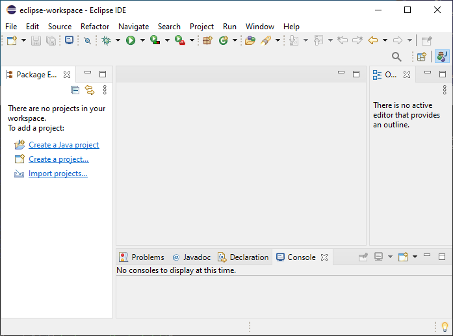
\includegraphics[]{images/EmptyEclipse}
\else
   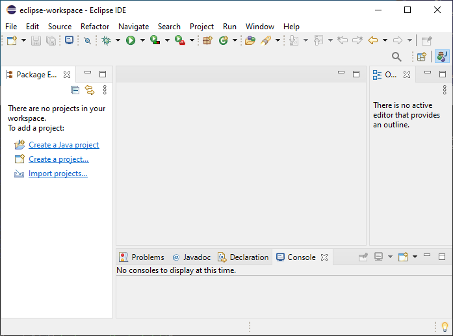
\includegraphics[width=0.7\textwidth]{images/EmptyEclipse}
\fi
\end{center}

\ifMacOS
\begin{sideblock}
Before closing Eclipse, you may want to pin its icon to your dock
to make it easier to restart.
\end{sideblock}
\fi

Newer versions of Eclipse come with their own version of
Java. However, since we want to use the Java 8 JDK, as discussed
above, we need to configure Eclipse to use that instead. This can be
done as follows:

\begin{enumerate}

\item From the main menu, select 
\ifMacOS
``{\sf Eclipse > Preferences...}''.
\else
``{\sf Window > Preferences}''.
\fi

\item A {\sf Preferences} dialog will open. In the left panel, select
``{\sf Java > Installed JREs}'', which will open an {\sf Installed JREs}
panel.
\ifMacOS % begin macOS
On MacOS, all installed JDKs {\it should} appear in the panel
including the Eclipse default and the JDK 8 which was just installed.
Click on the box to the left of the JDK 8 entry to select it;
ignore warnings about Java 15 compatibility. 
\else % begin Not macOS
Click the {\sf Add...} button at the right.

\item A {\sf JRE Type} dialog will appear. Leave ``Standard VM''
selected in the dialog and click {\sf Next}.

\item A {\sf JRE Definition} dialog will appear. In the ``{\sf JRE home}''
field at the top, enter the Java home \directory{} where Java 8 was
installed.
\ifWindows % begin Windows
On Windows, this is likely to be a location like {\tt C:\BKS Program
Files\BKS Java\BKS jdk1.8.0\_281}. Specifying the java
home \directory{} will cause some other fields to fill in
automatically, as seen here:
\begin{center}
\iflatexml
   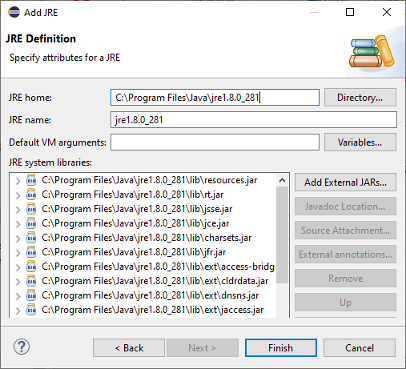
\includegraphics[]{images/EclipseJREDefinition}
\else
   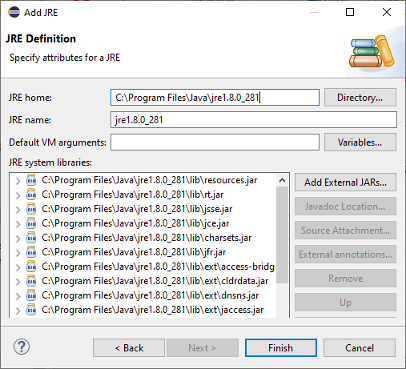
\includegraphics[width=0.6\textwidth]{images/EclipseJREDefinition}
\fi
\end{center}
\fi % end Windows

\item Click {\sf Finish}. Java 8 will now show up in the list of
installed JREs. 
\ifWindows % begin Windows
Click on the left box to select it, as shown
below (ignore any warnings about Java 15 compatibility).
\fi % end Windows 
\fi % end Not MacOS
\ifLinux % begin Linux
Click on the left box to select it; ignore any warnings about Java
15 compatibility.
\else % else NOT Linux
\begin{center}
\iflatexml
  \ifWindows
     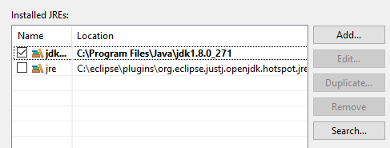
\includegraphics[]{images/EclipseInstalledJREs}
  \else
     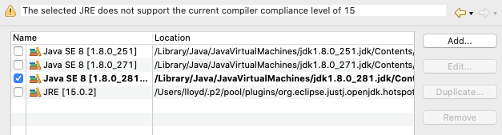
\includegraphics[]{images/EclipseInstalledJREsMacOS}
  \fi
\else
  \ifWindows
     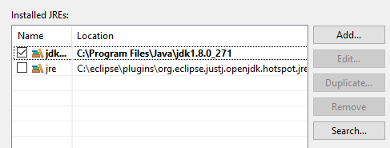
\includegraphics[width=0.6\textwidth]{images/EclipseInstalledJREs}
  \else
     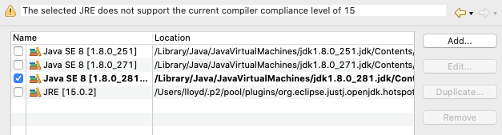
\includegraphics[width=0.8\textwidth]{images/EclipseInstalledJREsMacOS}
  \fi
\fi
\end{center}
\fi % end NOT Linux

\item Finish by clicking the ``{\sf Apply and Close}'' button at the
bottom of the {\sf Preferences} dialog.

\end{enumerate}

\section{Installing ArtiSynth}

You can now install ArtiSynth from GitHub. 

\begin{enumerate}

\item From the panel at the left of the main Eclipse frame, choose
``{\sf Import projects...}''. This will cause an {\sf Import} dialog to
appear, as shown below. Open ``{\sf Git > Projects from Git}'', and then
click {\sf Next}.

\begin{center}
\iflatexml
   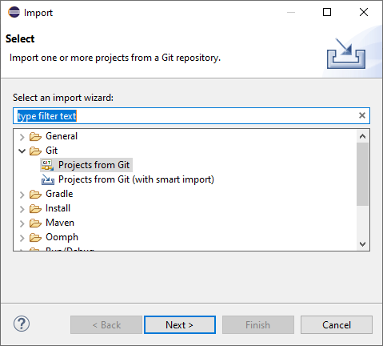
\includegraphics[]{images/EclipseImport}
\else
   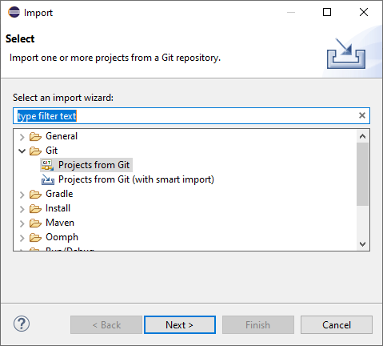
\includegraphics[width=0.6\textwidth]{images/EclipseImport}
\fi
\end{center}

\item In the next dialog, choose {\sf Clone URI}, and click {\sf Next}.

\item A {\sf Source Git Repository} dialog will appear, as shown
below. In the {\sf URI} field at the top, enter\\{\tt
https://github.com/artisynth/artisynth\_core.git}\\This will
automatically fill the {\sf Host} and {\sf Repository path} fields.
Click {\sf Next}.

\begin{center}
\iflatexml
   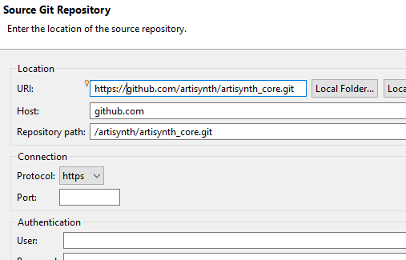
\includegraphics[]{images/EclipseGitRepoDialog}
\else
   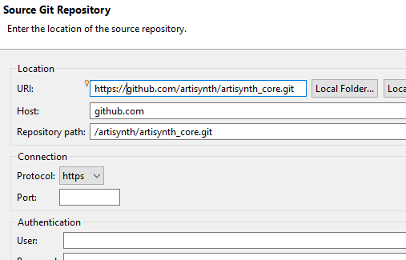
\includegraphics[width=0.6\textwidth]{images/EclipseGitRepoDialog}
\fi
\end{center}

\item A {\sf Branch Selection} dialog will appear; uncheck {\tt svn}, so
that only {\tt master} is selected. Click {\sf Next}. 

\item A {\sf Local Destination} dialog will appear, as shown below,
indicating the \directory{}into which ArtiSynth will be placed locally. Use
the default location, or edit it to some other desired location.  This
will be your {\it ArtiSynth installation \directory{}}.
Click {\sf Next}.

\begin{center}
\iflatexml
  \ifWindows
     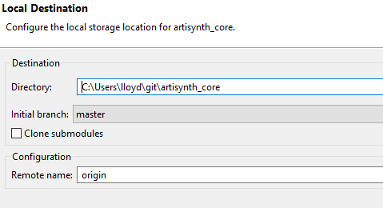
\includegraphics[]{images/LocalDestination}
  \else
     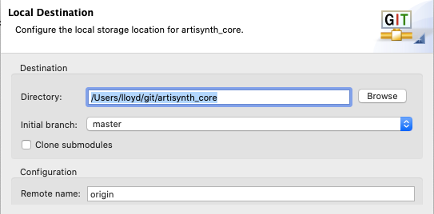
\includegraphics[]{images/LocalDestinationMacOS}
  \fi
\else
  \ifWindows
     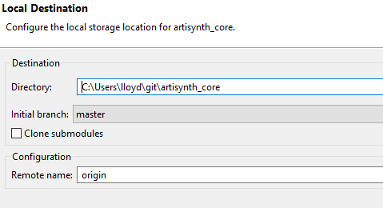
\includegraphics[width=0.55\textwidth]{images/LocalDestination}
  \else
     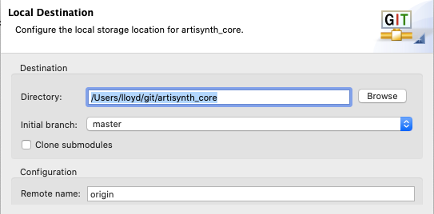
\includegraphics[width=0.55\textwidth]{images/LocalDestinationMacOS}
  \fi
\fi
\end{center}

\item ArtiSynth will now be downloaded; this may take a few minutes,
depending on your network connection speed. Another dialog will
appear, asking you to select to project import wizard.  Leave the
default (``{\sf Import existing Eclipse projects}'') selected, and
click {\sf Next}.

\item An {\sf Import Projects} dialog will appear, confirming that you
want to import {\tt artisynth\_core}. Leave everything as is, and
click {\sf Finish}.

\end{enumerate}

{\tt artisynth\_core} has now been imported into Eclipse as a
project. However, we are not quite done. Eclipse will try to compile
{\tt artisynth\_core}, but will fail because some Java and native
libraries are missing. (These libraries are not included in the
GitHub repository because they are quite large.) The compile failure
will be indicated by a red exclamation mark next to the {\tt
artisynth\_core} project entry in the Package Explorer:
%
\begin{center}
\iflatexml
   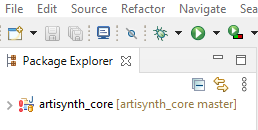
\includegraphics[]{images/artisynthBuildError}
\else
   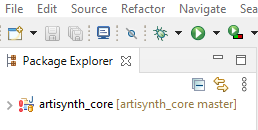
\includegraphics[width=0.35\textwidth]{images/artisynthBuildError}
\fi
\end{center}
%
The Java and native libraries must be downloaded separately, {\it
outside} of Eclipse.  
\ifWindows
Open a file explorer, navigate to the ArtiSynth installation folder
(e.g., {\tt C:\BKS people\BKS roger\BKS artisynth\_core}), open the
{\tt bin} \directory{}, and click on the {\tt updateArtisynthLibs}
batch file:
\begin{center}
\iflatexml
   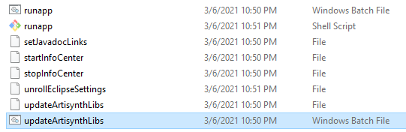
\includegraphics[]{images/UpdateArtisynthLibs}
\else
   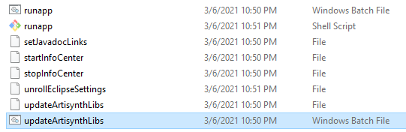
\includegraphics[width=0.65\textwidth]{images/UpdateArtisynthLibs}
\fi
\end{center}
This will load the libraries, temporarily displaying a terminal window
while doing so.
\else
Open a terminal window, change directories to the ArtiSynth
installation folder (e.g., {\tt /home/roger/artisynth\_core}), and run the
command\pdfbreak {\tt bin/updateArtisynthLibs}:
\begin{verbatim}
 > cd /home/roger/artisynth_core
 > bin/updateArtisynthLibs
\end{verbatim}
\fi
The process may take a few minutes, depending on network speed.

When the libraries are loaded, return to Eclipse, click on the {\tt
artisynth\_core} project to select it, then ``refresh'', either by
right clicking and selecting {\sf Refresh}, or by hitting the {\sf F5}
key. Eclipse should now find the libraries and compile ArtiSynth; a
green progress bar will appear at the lower right while compilation is
in progress.

\section{Running ArtiSynth}

You should now be able to run ArtiSynth. From the main menu, select
{\tt artisynth\_core} by clicking on it in the Package Explorer, and
then from the main menu select {\sf Run > Run}, and the ArtiSynth
application will start up (perhaps a little slowly the first time).
\ifMacOS

\begin{sideblock}
On older versions of {\tt MacOS}, errors similar to the following
may appear on the Eclipse Console output:
\begin{verbatim}
 2021-03-12 11:01:16.949 java[585:230b] invalid drawable 
\end{verbatim}
This is due to a problem in the default version of the Java-OpenGL
(JOGL) interface. To fix it, go back to the terminal window, and
from the ArtiSynth installation folder run the command
\begin{verbatim}
 > bin/installJOGL2.3.2
\end{verbatim}
Then return to Eclipse, select {\tt artisynth\_core} in the Package
Explorer, refresh it (right-click > {\sf Refresh} or {\sf F5}), and
wait for it to recompile.
\end{sideblock}

\fi
Within ArtiSynth, you can load a demonstration model by selecting
{\sf Models > Demos} from the main menu and choosing a demo model:

\begin{center}
\iflatexml
   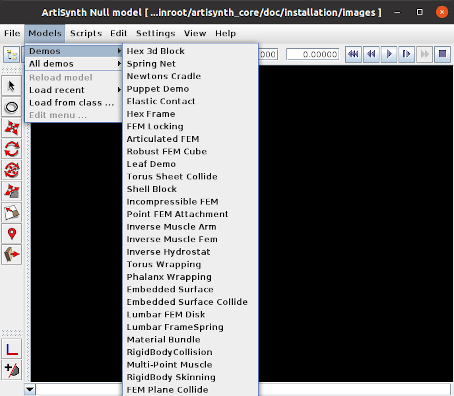
\includegraphics[]{images/ArtiSynthDemoMenu}
\else
   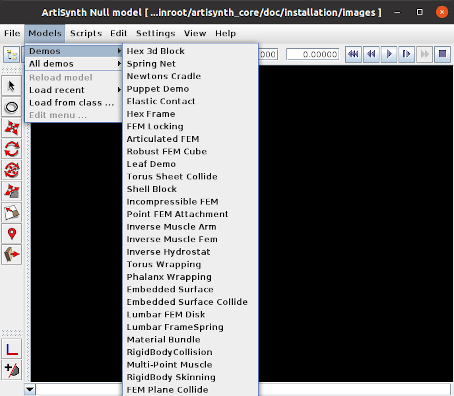
\includegraphics[width=0.75\textwidth]{images/ArtiSynthDemoMenu}
\fi
\end{center}

Once a model is loaded, it will appear in the viewer, and simulation
can be controlled using the ``play'' controls located at the upper right
of the application window:

\begin{center}
\iflatexml
  
\includegraphics[]{../uiguide/images/playControls}
\else
  
\includegraphics[width=2.5in]{../uiguide/images/playControls}
\fi
\end{center}

From left to right, these are: step size control, which controls the
simulation step size (in seconds); current simulation time (in
seconds); and the {\sf reset}, {\sf skip-back}, {\sf play/pause}, {\sf
single-step} and {\sf skip-forward} buttons.  Starting and stopping a
simulation is done by clicking {\sf play/pause}, and resetting it to
time 0 is done by clicking {\sf reset}.  The {\sf single-step} button
advances the simulation by one time step.

\ifMacOS

\begin{sideblock}
On newer versions of {\tt MacOS}, another problem that may occur when
trying to run ArtiSynth models is that MacOS may complain about using
a nonvalidated external library. This will take the form of a console
error that looks like this:
\begin{verbatim}
 ...
 /Users/lloyd/git/artisynth_core/lib/MacOS64/libPardisoJNI.11.1.2.1.dylib)
 not valid for use in process using Library Validation: library load disallowed
 by system policy 
 ...
\end{verbatim}
The problem here is that one or more of the native libraries are not
``known'' to Apple and are therefore not trusted. General information
on working around this problem is described here:

\href{https://support.apple.com/en-ca/HT202491}{support.apple.com/en-ca/HT202491}

The short version is to immediately open your Security and Privacy
settings after the error occurs, and then, near the bottom of the {\sf
General} tab, you should see a notification about the blocked
application with a button to the right labeled {\sf Open
Anyway}. Clicking that button will grant the application a security
exception.
\end{sideblock}

\fi

A model can also be loaded by specifying either its defining class or
a {\tt .art} file containing its textual representation.  For details,
see the section ``Loading, Simulating and Saving Models'' in
the \artisynthManual{uiguide}{ArtiSynth User Interface Guide}.  The
model menu can also be customized, as described in ``Customizing the
Model Menu''. The interface guide also contains information on using
the ArtiSynth GUI for model visualization, navigation, editing, and
simulation control. Instructions on how to build a model using Java
are given in the \artisynthManual{modelguide}{ArtiSynth Modeling
Guide}.

The image below shows ArtiSynth with the {\sf Spring Net} demo loaded:

\begin{center}
   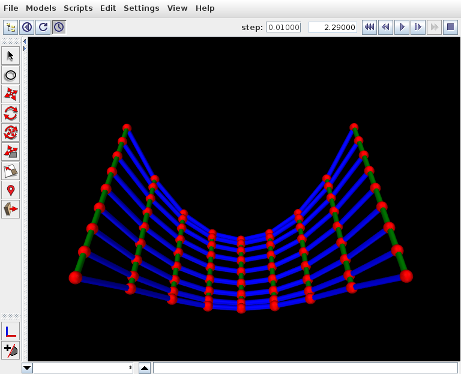
\includegraphics[width=0.60\textwidth]{images/SpringNetDemo}
\end{center}

\section{Making the Java JDK visible to your system}
\label{MakingJDKVisible:sec}

If the {\tt java} and {\tt javac} commands of your Java JDK are not
visible from a terminal command window, 
\ifWindows
you can fix this by adding
{\tt <JDK\_HOME>\BKS bin} to your system {\tt Path} variable, where
{\tt <JDK\_HOME>} is the installation \directory{} for your JDK. For example, if
your JDK is installed in {\tt C:\BKS Program Files\BKS Java\BKS
jdk1.8.0\_281}, you want to add {\tt C:\BKS Program Files\BKS
Java\BKS jdk1.8.0\_281\BKS bin} to the {\tt Path}, ahead of other
entries.

The {\tt Path} is a list of directories which the system searches in
order to find executables. You can add {\tt <JDK\_HOME>\BKS bin} 
to it as follows:

\subsection*{Windows 10}

\begin{enumerate}

\item Open the {\sf Start} search, enter ``{\tt env}'', and choose
{\sf ``Edit the system environment variables''}.

\item Click on {\sf Environment Variables}.

\item Under {\sf User variables} (the top window), click on {\sf Path}
and click {\sf Edit}. If {\sf Path} does not exist, click {\sf New}.

\item In the {\sf Edit environment variable} dialog, click {\sf New}
and enter {\tt<JDK\_HOME>\BKS bin}.

\item Close {\it all} dialogs by clicking {\sf OK} and restart 
any terminal windows.

\end{enumerate}

\subsection*{Windows 8 and earlier}

\begin{enumerate}

\item Right-click {\sf My Computer}, and then click {\sf Properties}.

\item Click the {\sf Advanced} tab.

\item Click {\sf Environment variables}.

\item In the top {\sf User variables} window, click on {\sf Path} and 
then {\sf Edit}. If {\sf Path} does not exist, click {\sf New}.

\item In the edit window, add {\tt<JDK\_HOME>\BKS bin} at the
left, separated from any following entries by a semi-colon '{\tt ;}'.

\item Close {\it all} dialogs by clicking {\sf OK} and restart 
any terminal windows.

\end{enumerate}
\fi
\ifMacOS
you can set the ``default'' JDK by setting the {\tt
JAVA\_HOME} environment variable.  This can be done inside the
initialization file for whichever command line shell you are using.

Assume that the desired JDK has version number {\tt 1.8.0\_281} and
that your home folder is {\tt <HOMEDIR>}.  Then for the {\tt bash}
shell, one can use a plain text editor to edit {\tt <HOMEDIR>/.bashrc}
and insert a line of the form
\begin{verbatim}
  export JAVA_HOME=`/usr/libexec/java_home -v 1.8.0_281`
\end{verbatim}
while for the {\tt csh} or {\tt tcsh} shells, one can edit {\tt
<HOMEDIR>/.cshrc} and insert a line of the form
\begin{verbatim}
  setenv JAVA_HOME `/usr/libexec/java_home -v 1.8.0_281`
\end{verbatim}

Setting {\tt JAVA\_HOME} can also be done directly within the shell;
doing it within the initialization file simply avoids the need to do
so each time a new terminal window is opened.
\fi
\ifLinux
then one fix is to add the \directory{} {\tt <JDK\_HOME>\SEP bin} to
your system {\tt PATH} variable, where {\tt <JDK\_HOME>} is the
installation \directory{} for your JDK.  In particular, {\tt
<JDK\_HOME>\SEP bin} should be added {\it ahead} of any other Java
installations that might be specified on the {\tt PATH}.  If you are
using the {\tt bash} shell, then modifications to {\tt PATH} can be
made inside the {\tt .bashrc} file located in your home directory.
For example, if {\tt <JDK\_HOME>} is {\tt /opt/java/jdk1.8.0\_281},
then you can add the line
\begin{verbatim}
export PATH="/opt/java/jdk1.8.0_281/bin:$PATH"
\end{verbatim}
to your {\tt .bashrc}. To see the current contents of the {\tt PATH},
open a terminal window and run the command
\begin{verbatim}
 > echo $PATH
\end{verbatim}
\fi

\end{document}
